\documentclass[11pt,a4paper]{article}

\usepackage[spanish,es-nodecimaldot]{babel}
\usepackage[utf8]{inputenc}
\usepackage[T1]{fontenc}
\usepackage{lmodern}
\usepackage{geometry}
\usepackage{graphicx}
\usepackage{booktabs}
\usepackage{array}
\usepackage{hyperref}
\usepackage{xcolor}
\usepackage{float}
\usepackage{enumitem}
\usepackage{tikz}
\usepackage{fancyhdr}
\usepackage{ragged2e}

\geometry{margin=2.5cm}
\hypersetup{colorlinks=true, linkcolor=blue, urlcolor=blue}
\graphicspath{{../Exploracion_Datos/Figuras/}}
\pagestyle{fancy}
\fancyhf{}
\fancyfoot[R]{\thepage}
\renewcommand{\headrulewidth}{0pt}
\renewcommand{\footrulewidth}{0pt}

\title{\textbf{Exploración de datos 1D y 2D}\\
\large Informe técnico -- Guía N°1}
\author{Gianfranco Giannoni\\
\small Herramientas para Ciencias de Datos (INFB6052)\\
\small Docente: Michael Miranda\\
\small Universidad Tecnológica Metropolitana}
\date{22 de octubre de 2026}

\begin{document}
\begin{tikzpicture}[remember picture,overlay]
\node[
  anchor=north west,
  xshift=1.5cm,
  yshift=-1.2cm
] at (current page.north west) {
\includegraphics[width=2.4cm]{logo_utem.png}};
\end{tikzpicture}
\begingroup
\centering
\vspace*{3.2cm}
{\LARGE\bfseries Exploración de datos 1D y 2D\par}
\vspace{0.35cm}
{\large Informe técnico -- Guía N°1\par}
\vspace{0.8cm}
{\large Gianfranco Giannoni\par}
\vspace{0.15cm}
{\normalsize Herramientas para Ciencias de Datos (INFB6052)\par}
{\normalsize Docente: Michael Miranda\par}
{\normalsize Universidad Tecnológica Metropolitana\par}
\vspace{0.35cm}
{\normalsize 22 de octubre de 2026\par}
\endgroup
\thispagestyle{empty}
\setcounter{page}{1}
\tableofcontents
\thispagestyle{empty}
\clearpage
\justifying

\section{Resumen}

Este informe documenta la exploración inicial de dos fuentes de datos con
estructura diferente: una señal 1D de audio musical y una imagen 2D asociada
a termografía de un sistema fotovoltaico. El objetivo es describir su
procedencia, representación numérica, unidades, calidad y limitaciones antes
de considerar cualquier aplicación de inteligencia artificial.

La señal de audio corresponde a un archivo WAV mono de 30 segundos, muestreado
a 22050 [Hz]. La imagen es un JPEG RGB de 640 por 512 píxeles. La exploración
confirma que ambas fuentes pueden cargarse y visualizarse reproduciblemente,
pero también muestra que sus valores no deben interpretarse automáticamente
como magnitudes físicas calibradas.

\section{Objetivos}

\begin{itemize}[leftmargin=*]
\item Verificar la carga y representación de una señal 1D y una imagen 2D.
\item Identificar ejes, unidades, resolución, canales y tipos numéricos.
\item Revisar indicadores básicos de calidad y consistencia.
\item Registrar procedencia, licencia, limitaciones y metadatos faltantes.
\item Proponer una pregunta de inteligencia artificial técnicamente validable.
\end{itemize}

\section{Fuentes y metodología}

\subsection{Señal 1D: GTZAN}

La señal utilizada es \texttt{musica\_bagpipe.wav}, una copia de trabajo del
dataset \emph{GTZAN music/speech collection}, disponible en
\href{https://www.kaggle.com/datasets/lnicalo/gtzan-musicspeech-collection}
{Kaggle} bajo licencia CC0.

Las muestras originales se representan como \(x[n]\). Para graficar se usa
una copia convertida a punto flotante y normalizada por el máximo representable
de \texttt{int16}; por tanto, la amplitud visualizada es relativa y no
corresponde a presión acústica real. El eje temporal se calcula como
\[
t[n] = \frac{n}{f_s}.
\]

\subsection{Imagen 2D: termografía fotovoltaica}

La imagen proviene del dataset \emph{Photovoltaic system thermography},
disponible en
\href{https://www.kaggle.com/datasets/marcosgabriel/photovoltaic-system-thermography}
{Kaggle} bajo licencia CC0. La copia de trabajo es un JPEG RGB de 640 por
512 píxeles. Su representación NumPy tiene forma
\(I[y,x,c]=(512,640,3)\) y tipo \texttt{uint8}.

Los canales \(c\) corresponden a rojo, verde y azul. Debido a que el archivo
no es una matriz radiométrica calibrada, sus valores entre 0 y 255 se
interpretan como intensidades codificadas. No es válido convertirlos
directamente a temperatura.

\subsection{Procedimiento}

La señal se cargó con herramientas de lectura de audio y la imagen con
Pillow. En ambos casos se inspeccionaron metadatos, dimensiones, tipo de
datos, rangos y valores no válidos. Se generaron gráficos con Matplotlib:
la señal completa y una vista ampliada de 0,1 segundos, junto con la imagen
original y un histograma independiente para cada canal RGB, para cada señal, respectivamente.

\section{Resultados}

\subsection{Señal de audio}

La señal contiene 661500 muestras, equivalentes a 30 segundos a 22050
muestras por segundo. El paso temporal esperado es
\(1/f_s=4.5351\times10^{-5}\) s y se verificó constante. No se encontraron
valores no finitos. La amplitud PCM (Modulación por impulsos codificados) observada va de -15756 a 16956; al
normalizar, el rango aproximado es de -0,481 a 0,517.

\begin{figure}[H]
\centering
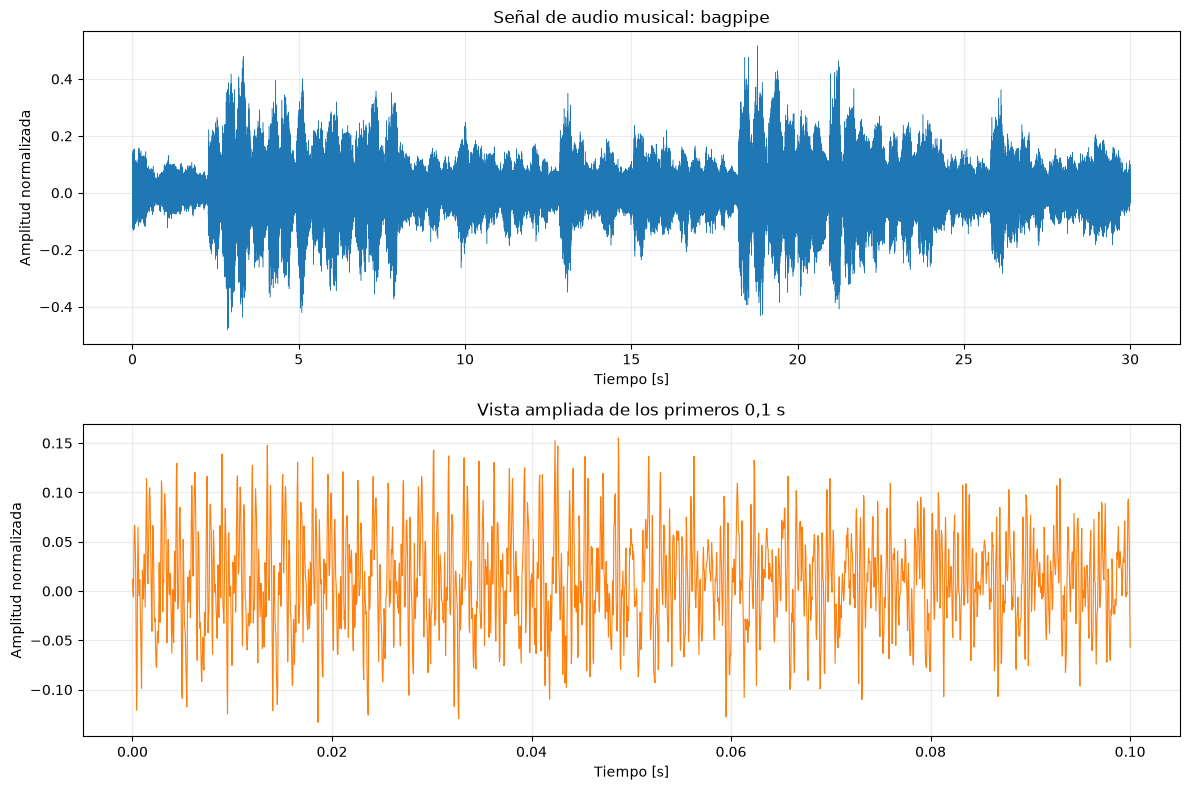
\includegraphics[width=\textwidth]{Figura 1A.png}
\caption{Señal de audio completa y vista ampliada de los primeros 0,1 s.}
\label{fig:audio}
\end{figure}

La figura 1 permite distinguir la envolvente temporal de la
señal completa y la variación muestra a muestra en la vista ampliada. La
amplitud no debe usarse para comparar niveles de grabación entre dispositivos
sin una calibración adicional.

\subsection{Imagen termográfica}

La imagen tiene formato JPEG, modo RGB, resolución 640 por 512 píxeles, tres
canales y tipo entero. El rango global observado es [15--237], sin
valores fuera de [0--255], sin canales constantes y sin saturación exacta en
los extremos 0 y 255.

\begin{figure}[H]
\centering
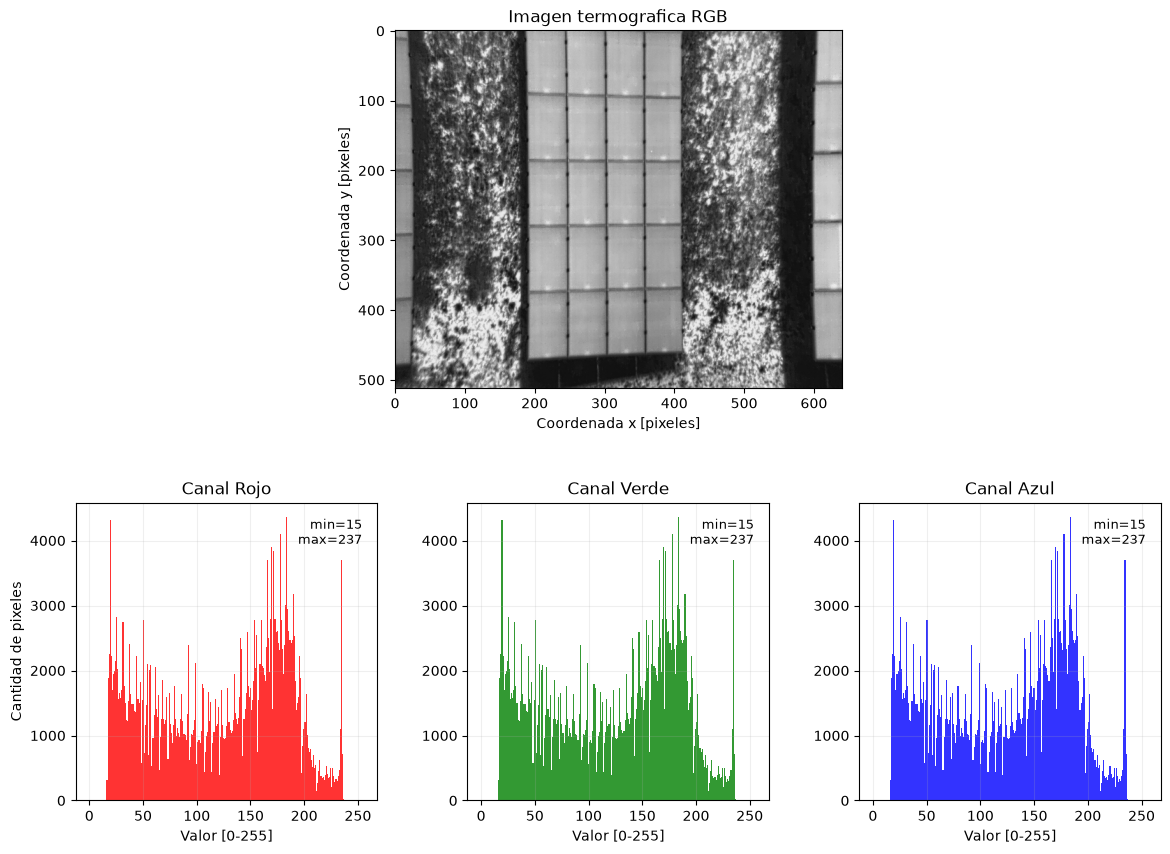
\includegraphics[width=.92\textwidth]{Figura 1B.png}
\caption{Imagen RGB y histogramas independientes de sus tres canales.}
\label{fig:imagen}
\end{figure}

Como se observa en la figura 2, los histogramas muestran la
distribución de intensidades codificadas. El parecido entre canales es
coherente con una imagen visualmente casi monocromática, pero no constituye
evidencia de igualdad de temperaturas ni permite diagnosticar una falla.

\section{Comparación y calidad}

\begin{table}[H]
\centering
\small
\begin{tabular}{p{.22\textwidth}p{.34\textwidth}p{.34\textwidth}}
\toprule
\textbf{Aspecto} & \textbf{Señal 1D} & \textbf{Imagen 2D}\\
\midrule
Fenómeno & Variación temporal de audio musical & Distribución espacial de intensidades\\
Estructura & Vector \(x[n]\) & Arreglo \(I[y,x,c]\)\\
Ejes & Tiempo en segundos y amplitud digital & Coordenadas en píxeles y canales RGB\\
Calidad observada & 661500 muestras, paso constante, 0 no finitos & 640$\times$512, rango válido, ningún canal constante\\
Limitación crítica & No hay presión acústica calibrada & No hay radiometría ni temperatura calibrada\\
\bottomrule
\end{tabular}
\caption{Comparación de las dos fuentes exploradas.}
\end{table}

En ambos casos la calidad de lectura es adecuada para una exploración inicial.
Sin embargo, la calidad computacional del archivo no equivale a calidad
metrológica. Para análisis de ingeniería se necesitarían metadatos de
adquisición y mediciones de referencia.

\section{Pregunta de inteligencia artificial}

La pregunta propuesta es: \textbf{¿puede un modelo identificar automáticamente
una posible anomalía térmica en un panel fotovoltaico a partir de una imagen,
manteniendo una tasa de falsos negativos aceptable frente a una inspección
experta?}

Para abordarla se requieren:
\begin{enumerate}[leftmargin=*]
\item etiquetas de normalidad, tipo de anomalía, ubicación y severidad;
\item temperaturas radiométricas calibradas, diferencias respecto de celdas
vecinas, potencia o corriente y resultado de inspección;
\item cámara, emisividad, distancia, ángulo, irradiancia, temperatura
ambiente, carga eléctrica y procedimiento de captura;
\item validación experta independiente y métricas como sensibilidad,
especificidad, precisión, falsos negativos y matriz de confusión.
\end{enumerate}

Con la imagen RGB disponible sólo puede realizarse exploración visual y
estadística. No debe afirmarse que un modelo mide temperatura o diagnostica
fallas sin recuperar las referencias físicas anteriores.

\section{Conclusiones}

La actividad permitió comprobar que una señal 1D se organiza principalmente
alrededor del tiempo, mientras que una imagen 2D se organiza alrededor de
coordenadas espaciales y canales. Ambos datos se cargaron, inspeccionaron y
visualizaron sin errores, conservando sus representaciones originales.

La principal conclusión metodológica es que la procedencia y las unidades son
parte del dato: normalizar un audio o visualizar una termografía RGB no crea
por sí mismo una medición física calibrada. Antes de entrenar un modelo se
deben ampliar las muestras, completar los metadatos, separar entrenamiento y
prueba y obtener validación experta.

\section*{Material complementario}

\begin{itemize}
\item Notebook de audio:
\href{../Exploracion_Datos/Notebooks/Actividad_A.ipynb}{Actividad\_A.ipynb}.
\item Notebook de imagen:
\href{../Exploracion_Datos/Notebooks/Actividad_B.ipynb}{Actividad\_B.ipynb}.
\item Ficha GTZAN:
\href{../Exploracion_Datos/Datos/Senal_1D/GTZAN/FUENTE.md}{FUENTE.md}.
\item Ficha termográfica:
\href{../Exploracion_Datos/Datos/Imagen_2D/PV_Termografia/FUENTE.md}{FUENTE.md}.
\end{itemize}

\end{document}
